\section{Datenbanksprachen}
 
MongoDB bietet verschiedene Möglichkeiten um Daten hinzuzufügen oder zu manipulieren. So können Dokumente beispielsweise über die Kommandozeile hinzugefügt werden. Zudem gibt es für viele Programmiersprachen einen Treiber, der in das jeweilige Projekt eingebunden werden kann. 
 
Da für diese Arbeit ein Programm in Java geschrieben wurde, kam der aktuelle mongo-java-driver in der Version 3.4.0 zum Einsatz. Allerdings sind die Kommandos für die Interaktion mit den Daten nicht sehr unterschiedlich zum normalen Kommandofenster. Nach der Wahl der Datenbank kann im Java Treiber  die entsprechende Collection ausgewählt und dieser anschliessend Dokumente hinzugefügt werden:
 
\begin{lstlisting}[basicstyle=\tiny]
MongoClient mongo = new MongoClient( "localhost" , 27017 );
MongoDatabase database = mongo.getDatabase("unidb");
MongoCollection<Document> stud = database
	.getCollection("studenten");
stud.drop();
studs.insertOne(new Document("Legi", 25403)
	.append("Name", "Jonas")
	.append("Semester", 12)
	.append("Hoeren", 5022));
mongo.close();
\end{lstlisting}

So wurde für die Testdaten ein Javaprogramm erstellt, dass alle Daten der UniDB in entsprechende Collections der MongoDB schreibt.

Für die Erwähnte Query, die in der Einführung bereits erwähnt wurde, wurde ein
separate Funktion geschrieben, die die Daten aus der Datenbank holt und aneinanderhängt. Darin wird für jeden Professor nachgeschlagen, welche Vorlesungen dieser hält. Anhand dieser wird die Anzahl SWS Punkte ermittelt, die der Professor unterrichtet. Zusätzlich wird gezählt, wie viele Studenten dieser Vorlesungen zuhören. Wenn die Query in MySQL ausgeführt wird, ist das Resultat folgendes:

\begin{figure}[h] 
	\centering
	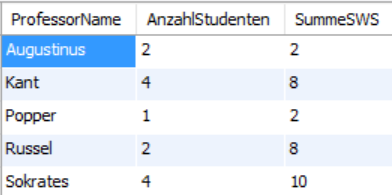
\includegraphics[width=0.5\textwidth]{./pictures/Query_MySQL_result.png}
	\caption{Query Resultat in MySQL}
	\label{fig:mysqlres}
\end{figure}

\newpage
Beim Javacode wird diese eine Tabelle angezeigt und mit einem Click auf den
Search Students Knopf wird besagte Funktion oben ausgeführt und die Tabelle
aktualisiert.
\begin{figure}[h]
	\centering
	\subfigure{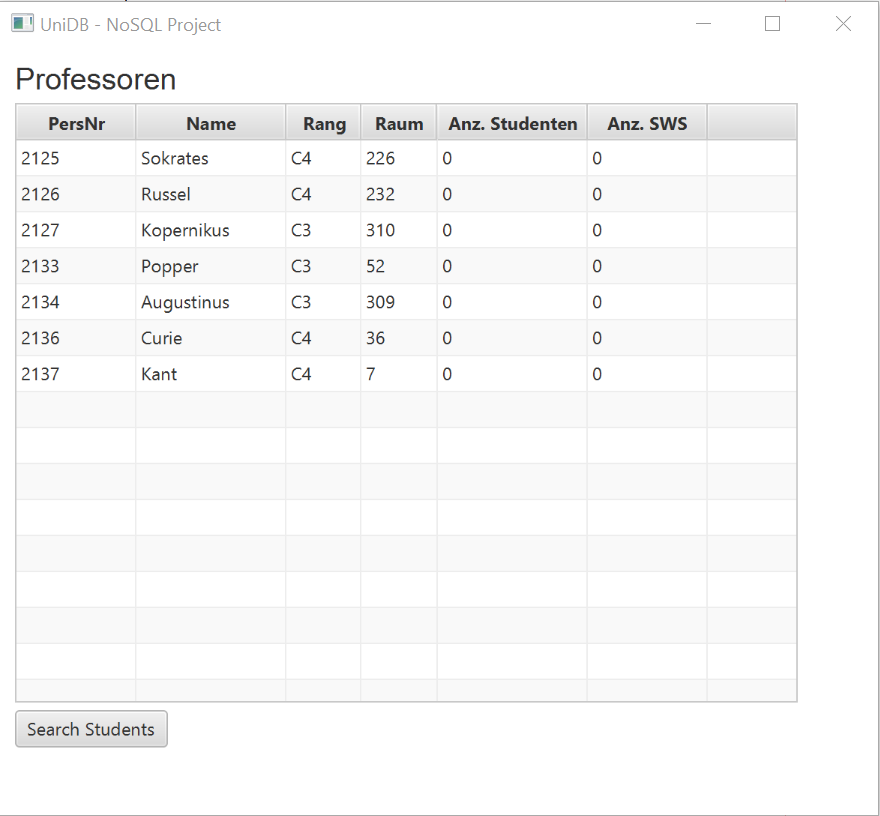
\includegraphics[width=0.49\textwidth]{./pictures/UniDBView.png}} 
	\subfigure{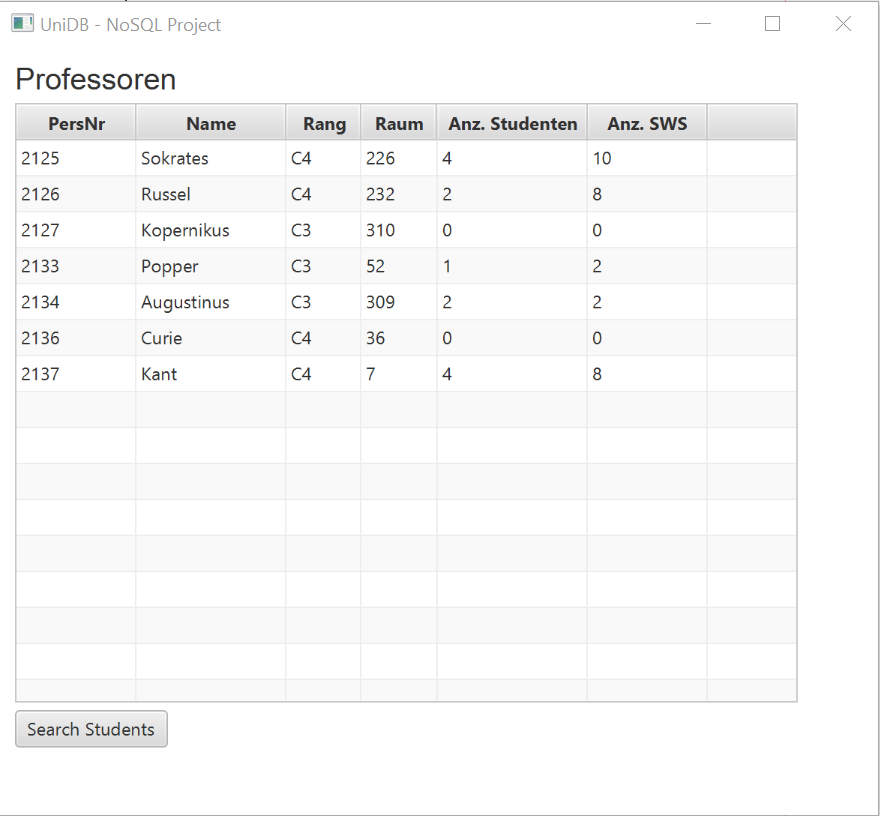
\includegraphics[width=0.49\textwidth]{./pictures/UniDBView_Query.png}} 
	\caption{Query Resultat MongoDB}
	\label{fig:monogdbres}
\end{figure}
